\section{Handling merge conflicts}
\begin{frame}[fragile]
    \slidetitle
  In this section you will learn to handle conflicts with:
  \begin{itemize}
\item difftool
\item mergetool
\item 3 way merge
\end{itemize}
\end{frame}

\subsection{A requirement change}
\begin{frame}[fragile]
    \subslidetitle
  Our customer changed his mind about the color of the green moon.
  \newline \vspace{1em}
  \#4 Change the color of the green moon to red.

  Implement the change in moon.js following this diff:
\begin{lstlisting}
(*\textcolor[HTML]{18B2B2}{@@ -4,7 +4,7 @@}*) var moons = [];
 init();
 moon( "blue" );
 moon( "white" );
(*\textcolor{red}{-}*)(*\textcolor{red}{moon( "green" );}*)
(*\textcolor[HTML]{00AA00}{+}*)(*\textcolor[HTML]{00AA00}{moon( "red" );}*)
 animate();
\end{lstlisting}

\end{frame}

\subsection{Display differences}
\begin{frame}[fragile]
    \subslidetitle
  The \cmd{git difftool} will run the application of your choice to display differences:
  \begin{lstlisting}
(*\textcolor[HTML]{18B2B2}{(master)}*) $ (*\textcolor[HTML]{0000AA}{git difftool --tool kdiff3}*)
Viewing (1/1): 'moon.js'
Launch 'kdiff3' [Y/n]: Y
\end{lstlisting}

  \vspace{1em}
  \centerline{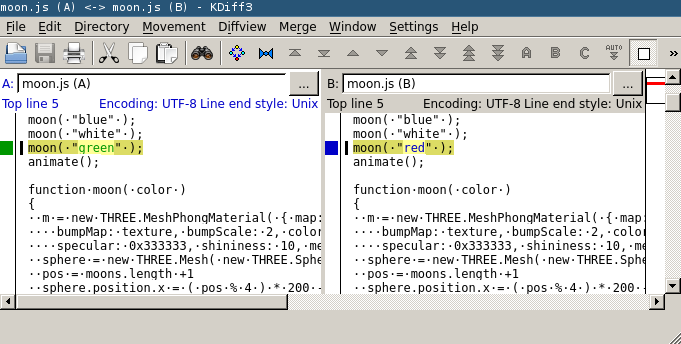
\includegraphics[width=10cm]{../screen/git-difftool-kdiff3.png}}

  Note: This can be helpful to call an external diff toll like kdiff3 or meld, especially to have a side-by-side diff.

\end{frame}


\subsection{Update feature-flag-color}
\begin{frame}[fragile]
    \subslidetitle
  Commit your changes on master:
\begin{lstlisting}
(*\textcolor[HTML]{18B2B2}{(master)}*) $ (*\textcolor[HTML]{0000AA}{git commit -a -m "change the green moon color to red, implements \#4"}*)
(*\textcolor[HTML]{18B2B2}{(master)}*) $ (*\textcolor[HTML]{0000AA}{git checkout feature-color-flag}*)
\end{lstlisting}

  Add a comment to the green moon like defined in the following diff:
  \begin{lstlisting}
(*\textcolor[HTML]{18B2B2}{@@ -4,7 +4,7 @@}*) var moons = [];
 init();
 moon( "blue" );
 moon( "white" );
(*\textcolor{red}{-}*)(*\textcolor{red}{moon( "green" );}*)
(*\textcolor[HTML]{00AA00}{+}*)(*\textcolor[HTML]{00AA00}{moon( "green" ); // no requirement}*)
 animate();
\end{lstlisting}

  Commit your changes:
  \begin{lstlisting}
(*\textcolor[HTML]{18B2B2}{(master)}*) $ (*\textcolor[HTML]{0000AA}{git commit -a -m "add comment about requirement for the green color"}*)
\end{lstlisting}
\end{frame}
\begin{frame}[fragile]
    \subslidetitle
\end{frame}

\subsection{git difftool}
\begin{frame}[fragile]
    \subslidetitle
\end{frame}

